% Preamble
\documentclass{aastex631}
\usepackage{natbib}
\usepackage{latexsym}
\usepackage{graphicx}
\usepackage{epsfig}
\usepackage{amssymb}
\usepackage{amsmath}
\usepackage{epstopdf}
\usepackage{hyperref}

%%%% Custom commands
\newcommand{\gradrad}{\ensuremath{\nabla_{\rm{rad}}}}
\newcommand{\gradad}{\ensuremath{\nabla_{\rm{ad}}}}
\newcommand{\Fbot}{\ensuremath{F_{\rm{bot}}}}
\newcommand{\Ftot}{\ensuremath{F_{\rm{tot}}}}
\newcommand{\Frad}{\ensuremath{F_{\rm{rad}}}}
\newcommand{\Fconv}{\ensuremath{F_{\rm{conv}}}}
\newcommand{\Fcz}{\ensuremath{F_{\rm{cz}}}}
\newcommand{\mP}{\ensuremath{\mathcal{P}}}
\newcommand{\dP}{\ensuremath{\delta_{\rm{p}}}}
\newcommand{\Lcz}{\ensuremath{L_{\rm{cz}}}}
\newcommand{\mR}{\ensuremath{\mathcal{R}}}
\newcommand{\mS}{\ensuremath{\mathcal{S}}}
\newcommand\Pran{\ensuremath{\mathrm{Pr}}}
\newcommand{\brunt}{Brunt-V\"{a}is\"{a}l\"{a}}

\newcommand{\angles}[1]{\langle #1 \rangle}
\newcommand{\pd}[1]{\partial_{#1}}
\renewcommand{\vec}[1]{\boldsymbol{#1}}
\newcommand{\M}[1]{\mathbf{#1}}
\renewcommand{\dot}{\vec{\cdot}}
\newcommand{\grad}{\vec{\nabla}}
\newcommand{\cross}{\vec{\times}}
\newcommand{\laplacian}{\nabla^2}

%%%% Journal preamble
\received{}
\revised{}
\accepted{}
\published{}
\submitjournal{ApJ}

\shorttitle{SHORT TITLE}
\shortauthors{Anders et al}


\begin{document}

%%%% Title and Abstract
\title{This is a title}
\author[0000-0002-3433-4733]{Evan H. Anders}
\affiliation{CIERA, Northwestern University, Evanston IL 60201, USA}
\author[0000-0001-5048-9973]{Adam S. Jermyn}
\affiliation{Center for Computational Astrophysics, Flatiron Institute, New York, NY 10010, USA}
\author[0000-0002-7635-9728]{Daniel Lecoanet}
\affiliation{CIERA, Northwestern University, Evanston IL 60201, USA}
\affiliation{Department of Engineering Sciences and Applied Mathematics, Northwestern University, Evanston IL 60208, USA}
\author[0000-0001-8935-219X]{Benjamin P. Brown}
\affiliation{Department Astrophysical and Planetary Sciences \& LASP, University of Colorado, Boulder, CO 80309, USA}

\correspondingauthor{Evan H. Anders}
\email{evan.anders@northwestern.edu}

\begin{abstract}
Blah Blah short description
\end{abstract}
\keywords{UAT keywords}



%%%% Body of paper
\section{Introduction}
\label{sec:introduction}
Convection is a crucial heat transport mechanism over some fraction of the stellar radius for all stars at some point in the stellar lifetime \citep{woosley_etal_2002, hansen_etal_2004, christensen-dalsgaard_2021}.
These motions drive the magnetic dynamo of the Sun and other stars \citep{brun_browning_2017}, leading to the host of emergent phenomena known as stellar activity.
Furthermore, convective motions impinge upon nearby stable layers, exciting gravity waves \citep{aerts2010}.
Convection is also responsible for mixing chemical compositions, which becomes increasingly important in the cores of evolved stars \citep{salaris_cassisi_2017}.
A complete and nuanced understanding is therefore crucial for understanding stellar structure, evolution, and observations.

One particular aspect of stellar convection which remains poorly understood even after decades of study is the class of mechanisms generally referred to as ``convective overshoot.''
Useful parameterizations of the way in which convective motions extend beyond the nominally Schwarzschild- or Ledoux- stable boundaries of the convective zone have historically been elusive.
Improved models of this ``overshoot'' could help to resolve many discrepancies between observations and theoretical model.
In the Sun and solar-type stars, better models of convective boundaries could help solve the mystery of low abundances of Li at the surface of solar-type stars \citep{pinsonneault1997, dumont_etal_2021}, the ``solar modeling problem'' \citep{basu_antia_2004, bahcall_etal_2005, zhang_li_2012, vinyoles_etal_2017, asplund_etal_2021} and problems in helioseismic profiles near the base of the convection zone \citep{christensen-dalsgaard_etal_2011}.
There is also ample evidence that we do not understand the nature of convective mixing at the boundary of core convection zones \citep{claret_torres_2018, jermyn_etal_2018, viani_basu_2020, martinet_etal_2021, pedersen_etal_2021} which could have profound implications for the post-main sequence evolution and remnants of massive stars \citet{farmer_etal_2019, higgins_vink_2020}.
In order to ensure that models can be evolved on fast (human) timescales, 1D stellar evolution codes rely on simple parameterizations of convective overshoot and mixing beyond convective boundaries \citep{shaviv_salpeter_1973, maeder1975, herwig2000, paxton_etal_2011, paxton_etal_2013, paxton_etal_2018, paxton_etal_2019}.
While some preliminary work has been done to couple 3D dynamical convective simulations with 1D stellar evolution codes \citep{jorgensen_weiss_2019}, these calculations are currently prohibitively expensive to perform e.g., at every timestep in a stellar evolution calculation.
In short, an improved theoretical understanding of the behavior of convective boundaries which can inform easy-to-calculate parameterizations is essential.

Convective overshoot and penetration have been studied in laboratory experiments and numerical simulations for decades, and has been reviewed by many authors \citep{marcus_etal_1983, zahn1991, browning_etal_2004, rogers_etal_2006, viallet_etal_2015, korre_etal_2019}.
%Early experiments of convective penetration of water in the laboratory \citep{deardorff_etal_1969} or simple numerical plumes \citep{schmitt_etal_1984} have given way to a wide array of dynamical experiments in recent years.
A slew of simulations in Cartesian \citep{musman1968, moore_weiss_1973, hurlburt_etal_1986, hurlburt_etal_1994, singh_etal_1995, saikia_etal_2000, brummell_etal_2002, rogers_glatzmaier_2005, kapyla_etal_2007, tian_etal_2009, andrassy_spruit_2015, kitiashvili_etal_2016, lecoanet_etal_2016, kapyla_etal_2017, couston_etal_2017, toppaladoddi_wettlaufer_2018, kapyla2019, cai2020} and spherical \citep{browning_etal_2004, rogers_etal_2006, brun_etal_2017, pratt_etal_2017, dietrich_wicht_2018, higl_etal_2021} geometry have been studied.
Despite this lengthy list of experiments, no consensus model of convective overshoot or penetration has emerged.
Throughout the remainder of this work, we will use terminology from this hydrodynamical literature.
``Convective penetration'' refers to convective motions which extend beyond the nominal Schwarzschild boundary of the convection zone \emph{and} flatten the temperature gradient towards the adiabatic.
``Convective overshoot'' refers to the motions that extend beyond the convective boundary but do not modify the thermal structure.
Our main focus in this paper will be on convective penetration.

\citet{zahn1991} theorized that convective penetration should depend only on how steeply the radiative temperature gradient varies at the convective boundary.
Some simulations \citep{hurlburt_etal_1994, rogers_etal_2006} have shown at least partial agreement with this theory.
A semianalytic model of solar overshoot \citep{rempel2004} also agreed with the early ideas of Zahn. 
Furthermore, some select simulations have found hints that convective overshoot or penetration may be sensitive the magnitude of the flux in some way \citep{singh_etal_1998, hotta2017, kapyla2019}.
These results suggest that the gradients of fluxes near convective boundaries deserve further examination.

In this work, we design two numerical experiments to test the theory of \citet{zahn1991}.
We use a modified incompressible, Boussinesq model to study the simplest possible system, and re-derive his theory in our simplified limit.
The results of our simulations are in full agreement with Zahn's theory.
\begin{quote}
\emph{
Specifically, we find that the depth of convective penetration depends on the gradient of the radiative flux near the convective boundary.
}
\end{quote}
Thus, the penetration depth can be approximated so long as the radiative conductivity, or likewise the opacity, is known at the convective boundary.

We present these findings as follows.
In Sec.~\ref{sec:theory}, we describe our modified Boussinesq equations, re-derive the theory of \citet{zahn1991}, and retrieve predictions for our two experimental designs from that theory.
In Sec.~\ref{sec:simulation_details}, we describe our simulation setup and parameters.
In Sec.~\ref{sec:results}, we present the results of these simulations, with a particular focus on the depth of the penetrative regions.
In Sec.~\ref{sec:solar_model}, we create and discuss a solar MESA model which uses this theory to determine the bottom of the solar convection zone.
Finally, we discuss how future simulations can put finer constraints on this theory in Sec.~\ref{sec:discussion}.

\section{Theory}
\label{sec:theory}
Throughout this work, we will utilize a modified version of the Boussinesq equations of motion, similar to the model derived by \citet{spiegel_veronis_1960} and utilized by e.g., \citet{korre_etal_2019}.
In dimensional form,
\begin{align}
&\grad\dot\vec{u} = 0 
\label{eqn:incompressible} \\
&\partial_t \vec{u} + \vec{u}\dot\grad\vec{u} = -\frac{1}{\rho_0}\grad p + \frac{\rho'}{\rho_0}\vec{g} + \nu\grad^2 \vec{u} 
\label{eqn:momentum} \\
&\partial_t T + \vec{u}\dot\grad T + w \gradad + \grad\dot[-k \grad \overline{T}] = \chi\grad^2 T' + Q
\label{eqn:temperature} \\
&\frac{\rho'}{\rho_0} = -|\alpha| T.
\label{eqn:boussinesq}
\end{align}
In this model, $\rho_0$ is a (constant) background density and $\rho'$ are fluctuations which act only in the buoyancy force and varies linearly with the temperature $T$ according to the coefficient of thermal expansion, $\alpha = \partial\ln\rho / \partial T$.
Furthermore, $\vec{u}$ is the velocity vector, $\nu$ and $\chi$ are respectively the viscous and thermal diffusivity, $Q$ is a bulk internal heating term \citep[as in e.g.,][]{goluskin_vanderpoel_2016}, and $\gradad$ is the adiabatic temperature gradient (we define $\gradad$ as a positive value to align with stellar structure conventions; this means marginal stability is achieved when $\partial_z T = -\gradad$).
We modify the model of \citet{spiegel_veronis_1960} to allow the mean temperature profile $\overline{T}$ to carry a radiative flux $\Frad = -k \grad \overline{T}$, where $k$ is a radiative diffusivity which can vary with height.
We assume that the classical thermal diffusion term $\chi \grad^2 T'$  only acts on the fluctuations away from the mean temperature profile, $T' \equiv T - \overline{T}$.

The basis of the theory of \citet{zahn1991} is that the size of the convection zone is determined by the horizontally-averaged energetics and buoyancy breaking.
We assume convection reaches a time-stationary, equilibrium state; we vertically integrate Eqn.~\ref{eqn:temperature} and take a horizontal average to find
\begin{equation}
\Ftot = \Frad + \Fconv = \int Q dz + \Fbot,
\end{equation}
with $\Fconv = \overline{w T}$ and $\Fbot$ the flux at the bottom of the convective domain and $\Ftot$ the total flux, which can vary in height according to integral of $Q$.
We next assume that convection penetrates above the nominal schwarzschild boundary of the convection zone and mixes the temperature gradient towards the adiabatic in that region.
Thus, in that region, the convective flux can be found,
\begin{equation}
\Fconv = \Ftot - F_{\rm{rad, ad}} = \Ftot - k \grad_{\rm{ad}}.
\end{equation}
By definition, in this region, $\grad_{\rm{ad}} > \grad_{\rm{rad}}$, where $\grad_{\rm{rad}} = \Ftot/k$, so this requires that $\Fconv < 0$ in the convective penetration region.
We next assume that the temperature and velocity are highly correlated in the penetrative region with very similar horizontal fluctuations,
\begin{equation}
w(x,y,z) = W(z)h(x,y),
\qquad
T'(x,y,z) = \delta T(z)h(x,y).
\end{equation}
We here assume that $\overline{h} = 0$ and $\overline{h^2} \neq 0$.
We can then express the convective flux in terms of these vertically-varying profiles and an average over the horizontal structure of the flows,
\begin{equation}
\Fconv \equiv \overline{w T} = \overline{h^2} \, W(z) \, \delta T(z).
\label{eqn:Fconv_vertical}
\end{equation}
In the penetrative region, since $\Fconv < 0$, $W(z)$ and $\delta T(z)$ must be oppositely signed and the convective flows should eventually come to a stop through buoyancy breaking.
This is achieved through a balance between advection and buoyancy in the vertical momentum equation (Eqn.~\ref{eqn:momentum} with Eqn.~\ref{eqn:boussinesq}), 
\begin{equation}
\frac{1}{2}\frac{d w^2}{dz} = |\alpha| g T'.
\end{equation}
Multiplying both sides by $h(x,y)$, taking a horizontal average, and then substituting $\delta T(z)$ using Eqn.~\ref{eqn:Fconv_vertical}, we retrieve a simple ordinary differential equation,
\begin{equation}
\frac{\overline{h^3}}{6 |\alpha| g \overline{h^2}} dW^3 = \Fconv dz.
\label{eqn:theory_ode}
\end{equation}
This equation can be integrated over the depth of the convection zone from $W = 0$ to $W = W_0$ at the convective boundary, as well as over the penetration zone from $W = W_0$ to where $W = 0$.
We assume however that the horizontal structure $h$ of the flux-carrying flows is not identical in the convection zone (CZ) and the penetration zone (PZ).
Integrating Eqn.~\ref{eqn:theory_ode} over the CZ and PZ and taking a ratio of these two equations, we find
\begin{equation}
-\frac{(\overline{h}^3/\overline{h^2})_{\rm{PZ}}}{(\overline{h^3}/\overline{h^2})_{\rm{CZ}}} = 
\frac{\int_{\rm{PZ}} \Fconv dz}{\int_{\rm{CZ}} \Fconv dz}.
\label{eqn:theory_fraction}
\end{equation}
In order to move further with this theory, it is necessary to specify the vertical shape of $\Fconv$, which is in turn set by $Q$, $\gradad$, and $k$.
We will assume that $\gradad$ has a constant value and that the internal heating $Q$ is localized near the bottom of the CZ so that a constant convective flux $\Fcz$ is carried in the bulk convection zone.
As a result, the vertical profile of $\Frad$ and $\Fconv$ is determined completely by the behavior of $k(z)$ near the convective boundary.
We will study two cases in this work: a discontinuous jump in $k(z)$ at the convective boundary, and a piecewise-linear profile of $k(z)$ whose derivative may be discontinuous at the convective boundary.

\subsection{Case I: Discontinuous radiative conductivity}
\label{sec:discontinuous_theory}
We first consider a radiative conductivity $k(z)$ which is discontinuous, with a value of $k_{\rm{CZ}}$ in the convection zone and larger value $k_{\rm{RZ}}$ in the PZ and radiative zone (RZ).
The values of $k$ are chosen so that the convective flux follows
\begin{equation}
\Fconv(z) = \begin{cases}
\Fcz			&	z \leq \Lcz,\\
-\mP_D^{-1} \Fcz & 	z > \Lcz 
\end{cases}.
\end{equation}
Here, $\mP_D^{-1}$ is the ``penetration parameter'' (subscript D for discontinuous case).
Plugging this functional form of the flux into Eqn.~\ref{eqn:theory_fraction}, and integrating the convection zone from $z = 0$ to $z = \Lcz$ and the penetration zone from $z = \Lcz$ to $z = \Lcz + \dP$,
\begin{equation}
\frac{\dP}{\Lcz} = \mP_D
\frac{(\overline{h}^3/\overline{h^2})_{\rm{PZ}}}{(\overline{h^3}/\overline{h^2})_{\rm{CZ}}}.
\label{eqn:discontinuous_prediction}
\end{equation}
We then see that the size of the penetration region is linearly proportional to $\mP_D$ and is a function of the horizontal structure of the convective dynamics in the PZ and the CZ.
This makes sense; As $\mP_D$ grows, the magnitude of $\Fconv$ in the PZ shrinks, and so too does the breaking force of buoyancy.

\subsection{Case II: Piecewise linear radiative conductivity}
\label{sec:linear_theory}
We next assume that $k(z)$ is not discontinuous at the CZ-PZ boundary, but that its derivative may be.
As a result, the convective flux in the vicinity of the boundary takes the form
\begin{equation}
\Fconv(z) = 
\begin{cases}
(\partial_z k)_{\rm{cz}}\gradad (\Lcz - z) & z \leq \Lcz \\
-\mP_L^{-1}(\partial_z k)_{\rm{cz}}\gradad (z - \Lcz) & z > \Lcz
\end{cases},
\end{equation}
where we assume that $(\partial_z \Frad)_{\rm{cz}} =  (\partial_z k)_{\rm{cz}}\gradad$ is a constant.
Again, solving Eqn.~\ref{eqn:theory_fraction} with this functional form of the flux, we retrieve
\begin{equation}
\frac{\dP}{\Lcz} = \sqrt{\mP_L
\frac{(\overline{h}^3/\overline{h^2})_{\rm{PZ}}}{(\overline{h^3}/\overline{h^2})_{\rm{CZ}}}},
\label{eqn:linear_prediction}
\end{equation}
which is identical to the prediction of \citet{zahn1991} when we take $\mP_L = 1$.
In this work, we will test the predictions of Eqns.~\ref{eqn:linear_prediction} and \ref{eqn:discontinuous_prediction}.
Our aim is to see if the predicted scalings with $\mP$ are realized in direct numerical simulations, and to measure preliminary values for $\frac{(\overline{h}^3/\overline{h^2})_{\rm{PZ}}}{(\overline{h^3}/\overline{h^2})_{\rm{CZ}}}$ in local simulations.

\section{Simulation Details}
We nondimensionalize Eqns.~\ref{eqn:incompressible}-\ref{eqn:boussinesq} on the length scale of the convection zone, the timescale of freefall across that convection zone, and the temperature scale of the internal heating over that freefall time,
\begin{equation}
\begin{split}
&T^* = (\Delta T)T = Q_0 \tau T,\qquad
\partial_{t^*} = \tau^{-1}\partial_t = \left(\frac{\alpha g Q_0}{\Lcz}\right)^{1/3} \partial_t,\qquad
\grad^* = \Lcz^{-1} \grad,\qquad
\vec{u}^* = u_{\rm{ff}}\vec{u} = \left(\alpha g Q_0 \Lcz^2\right)^{1/3}\vec{u},
\\
&k^* = (\Lcz^2 \tau^{-1})k,\qquad
Q^* = Q_0 Q,\qquad
\mR = \frac{u_{\rm{ff}} \Lcz}{\nu},\qquad
\Pran = \frac{\nu}{\chi}.
\end{split}
\end{equation}
Here, quantities with $*$ (e.g., $T^*$) refer to the ``dimensionful'' quantities of Eqns.~\ref{eqn:incompressible}-\ref{eqn:boussinesq}, and going forward quantities without these (e.g., $T$) will be dimensionless.
The equations of motion are therefore
\label{sec:simulation_details}
\begin{align}
&\grad\dot\vec{u} = 0 
\label{eqn:nondim_incompressible} \\
&\partial_t \vec{u} + \vec{u}\dot\grad\vec{u} = -\grad \varpi + T \hat{z} + \mR^{-1}\grad^2 \vec{u}
\label{eqn:nondim_momentum} \\
&\partial_t T + \vec{u}\dot\grad T + w \grad_{\rm{ad}}  + \grad\dot[-k \grad \overline{T}] = (\Pran\mR)^{-1}\grad^2 T' + Q.
\label{eqn:nondim_temperature}
\end{align}
We construct a domain in the range $z \in [0, L_z]$ where in this work we choose $L_z \geq 2$ so that the domain contains at least two convection zone length scales according to the Schwarzschild criterion.
We decompose the temperature field into a background and fluctuations, $T(x, y, z, t) = T_0(z) + T_1(x, y, z, t)$.
For boundary conditions, we impose impenetrable, no-slip boundary conditions at the top and bottom of the box so that $\vec{u} = 0$ at $z = [0, L_z]$.
We also impose a fixed-flux boundary at the bottom of the box ($\partial_z T_1 = 0$ at $z = 0$) and a fixed temperature boundary at the top of the domain ($T_1 = 0$ at $z = L_z$).

We impose a constant internal heating which spans only part of the convection zone,
\begin{equation}
Q = \begin{cases}
0		& z < 0.1\,\,\rm{or}\,\,z\geq 0.1 + \delta_H,\\
|Q_{\rm{mag}}|		& 0.1 \leq z \leq 0.1 + \delta_H
\end{cases}.
\end{equation}
The integrated value of the flux through the system from the heating is therefore $F_H(z > 0.1 + \delta_H) = \int_0^z Q_{\rm{mag}} dz = Q_{\rm{mag}}\delta_H$.
Throughout this work we choose $Q_{\rm{mag}} = 1$ and $\delta_H = 0.2$ so $F_H = 0.2$.
We offset this heating from the bottom boundary to $z = 0.1$ to avoid heating within the bottom impenetrable boundary layer where velocities go to zero and $k$ is small; this prevents strong temperature gradients from establishing there.
We assume that the (adiabatic) temperature gradient at the bottom boundary carries some flux, $\Fbot = \zeta F_H$ and we choose $\zeta = 10^{-3}$ so that most of the flux in the convection zone is carried by the convection.

In our equations, we expect the volume-average convective velocities to depend on the magnitude of the heating, $\angles{\vec{u}} \approx Q_{\rm{mag}}^{1/2} \approx 1$, so the characteristic convective frequency $f_{\rm{conv}} \approx \angles{\vec{u}} \Lcz \approx 1$.
We want to allow the stiffness of the radiative-convective interface to be a control parameter.
The stiffness is defined,
\begin{equation}
\mS \equiv \frac{N^2}{f_{\rm{conv}}} \approx N^2,
\end{equation}
where $N^2$ is the \brunt$\,$frequency in the radiative zone.
In our nondimensionalization, $N^2 = \gradad - \gradrad$ where $\gradrad = \Ftot/k$, so by choosing a value of the stiffness we set the magnitude of the background temperature gradient, $T_0$ which in turn sets the value of $k$ in the radiative zone.

The crucial place in which our model differs from that of prior work is that we define a ``penetration parameter,'' $\mP$, which determines the size of the convective penetration region.
We define
\begin{equation}
\mP = -\frac{\Fconv|_{\rm{CZ}}}{\Fconv|_{PZ}},
\end{equation}
where $\Fconv|_{PZ}$ is the negative convective flux carried in a perfectly adiabatic convective penetration region.
We construct our experiments so that $\mP$ and $\mS$ can be varied separately.
We suspect that many past experiments have implicitly set $\mP \approx \mS^{-1}$.

Aside form $\mS$ and $\mP$, the two remaining control parameters that control our experiments determine the degree of turbulence.
The value of $\mR$ roughly corresponds to the value of the peak Reynolds number measured in the simulations, and we set the ratio of the diffusivities $\Pran = 0.5$ throughout this work.
Astrophysical convection is in the limit of $\Pran \ll 1$; we choose a modest value of $\Pran$ which slightly separates the scales between thermal and viscous structures while still allowing us to achieve convection with large Reynolds and P\'{e}clet numbers.

\subsection{Case I: Discontinuous radiative conductivity}
Most of the simulations in this paper study simulations with a discontinuous radiative conductivity,
\begin{equation}
k_D(z) = \begin{cases}
k_{\rm{CZ}}	&	z < 1 \\
k_{\rm{RZ}} &	z \geq 1
\end{cases}.
\end{equation}
Leaving $\mS$ and $\mP_D$ as free parameters and requiring that the adiabatic gradient can carry the $\Fbot$ at $z = 0$ and that the radiative gradient can carry the flux for $z \geq 1$ specifies this system fully,
\begin{equation}
k_{\rm{RZ}} = \frac{\delta_H}{\mS\mP_D},\qquad
k_{\rm{CZ}} = k_{\rm{RZ}}\frac{1}{1 + \zeta + \mP_D^{-1}},\qquad
\gradad = Q_{\rm{mag}}\mS\mP_D(1 + \zeta + \mP_D^{-1}),\qquad
\gradrad = \gradad - Q_{\rm{mag}}\mS.
\end{equation}

We study three sweeps through the ($\mP_D$, $\mS$, $\mR$) parameter space in this paper (one in which we vary each parameter while holding the other parameters constant).
We use ``Reference values'' of $\mP_D = 4$, $\mS = 10^3$, and $\mR = 400$; all of our parameter space sweeps pass through this point in the three-dimensional parameter space.
As in section \ref{sec:discontinuous_theory}, we expect $\delta_p \propto \mP_D$.

\subsection{Case II: Piecewise linear radiative conductivity}
We additionally study a select few simulations where the radiative conductivity's gradient is piecewise discontinuous,
\begin{equation}
\partial_z k = \partial_z k_0
\begin{cases}
1	&	z < 1 \\
\mP_L^{-1} &	z \geq 1
\end{cases}
\end{equation}
Since $k$ varies with height, the value of $\mS$ and $\mP$ also vary with height; we specify their values at $z = 2$.
by this choice, we require
\begin{equation}
\partial_z k_0 = \frac{\delta_H}{\Lcz \mS \xi},\qquad
k_b = \frac{\delta_H\zeta}{\mS\xi},\qquad
\gradad = Q \mS \xi,
\end{equation}
where $\xi \equiv 1 + \mP_L(1 + \zeta)$.
In these simulations, we hold $\mS = 10^3$ and $\mR = 800$ while varying $\mP_L$.
As in section \ref{sec:linear_theory}, we expect $\delta_p \propto \mP_L^{1/2}$.

\subsection{Numerics}
We time-evolve equations \ref{eqn:nondim_incompressible}-\ref{eqn:nondim_temperature} using the Dedalus pseudospectral solver \citep{burns_etal_2020}\footnote{we use X version} using timestepper RK443 \citep{ascher_etal_1997}.
All fields are represented as spectral expansions of $n_z$ Chebyshev coefficients in the vertical ($z$) direction and as ($n_x$,$n_y$) Fourier coefficients in the horizontal ($x$,$y$) directions; our domains are therefore horizontally periodic.
The aspect ratio of our domains is two so that $x \in [0, L_x]$ and $y \in [0, L_y]$ with $L_x = L_y = 2 L_z$.
To start our simulations, we add random noise temperature perturbations with a magnitude of $10^{-3}$ to a background temperature profile $\overline{T}$; we discuss the choice of $\overline{T}$ in appendix \ref{app:accelerated_evolution}.
We produce the figures in this paper using matplotlib \citep{hunter2007, mpl3.3.4}.
All of the Python scripts used to run the simulations in this paper and to create the figures in this paper are publicly available in a git repo, found at [CITE].

We can't use true discontinuities and so we use approximate Heaviside functions like follows (TODO).

\subsection{Penetration depth measurements}

\section{Results}
\label{sec:results}

\subsection{Qualitative description of simulation evolution}

\begin{figure}[t!]
\centering
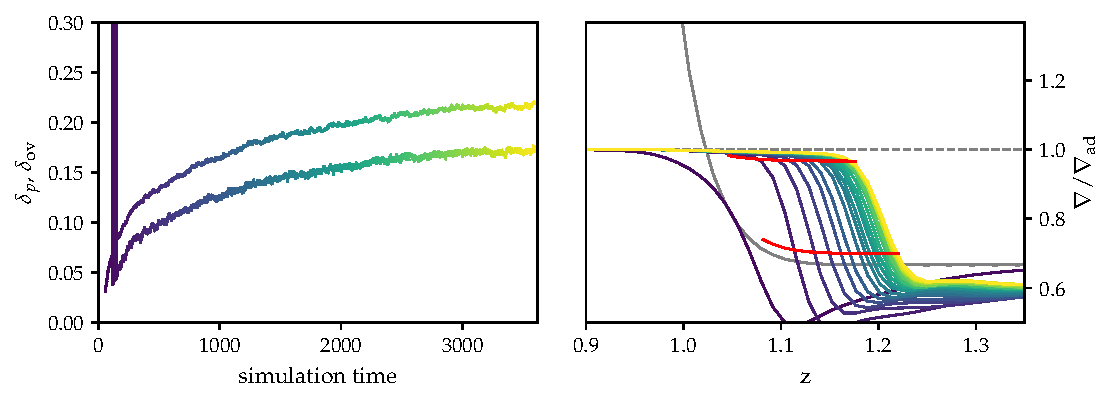
\includegraphics[width=\textwidth]{time_evolution.pdf}
\caption{(Top panel) we show traces of the time evolution of the points in the simulation where $\grad$ has departed from $\gradad$ by 10\% (bottom curve) and 90\% (top curve) of $\Delta = \gradad - \gradrad$.
Time is plotted on the x-axis in freefall units which are roughly equal to convective overturn times; the color of the line represents the simulation time.
While this evolution is initially fast (changing noticeably over hundreds of overturn times), as the convection zone approaches its final size its evolution drastically slows down.
(Bottom panel) The vertical profile of $\grad/\gradad$ is plotted against height at different times (where the color denotes the time and matches the color of the top panel.
The (constant) value of $\gradad$ is denoted by the horizontal dashed grey line, and the value of $\gradrad$ is denoted by the solid grey line.
The 10\% and 90\% departure curves from the top panel are overplotted as red lines.
\label{fig:time_evolution}
}
\end{figure}

In Fig.~\ref{fig:time_evolution}, we show the time evolution of a Case I simulation with $\mR = 400$, $\mS = 10^3$, and $\mP_D = 2$ (TODO: change to 4) whose initial conditions set $\grad = -\partial_z T$ equal to $\gradad$ in the convection zone ($z < 1$) and equal to $\gradrad$ in the radiative zone ($z > 1)$.
Initially, over hundreds of overturn times, the front of the convection zone drastically advances past the Schwarzschild boundary of the convection zone at $z = 1$.
As the convection zone advances and mixes $\grad \rightarrow \gradad$ within itself; this steepening of $\grad$ within the PZ is accompanied by a flattening of $\grad < \gradrad$ at the base of the RZ along the front of the CZ.
This flattening of $\grad$ increases the value of $N^2 = \gradad - \grad$ at the front of the convection zone, slowing the advancement of the convection zone until this disequilibrium state diffuses to the top boundary of the simulation.
This stiffer radiative-convective interface, combined with the presence of an increasingly growing breaking region in the form of the PZ slows the advancement of the convective front and the final equilibration of the top boundary of the convection zone takes thousands of convective overturn times.

\begin{figure}[t!]
\centering
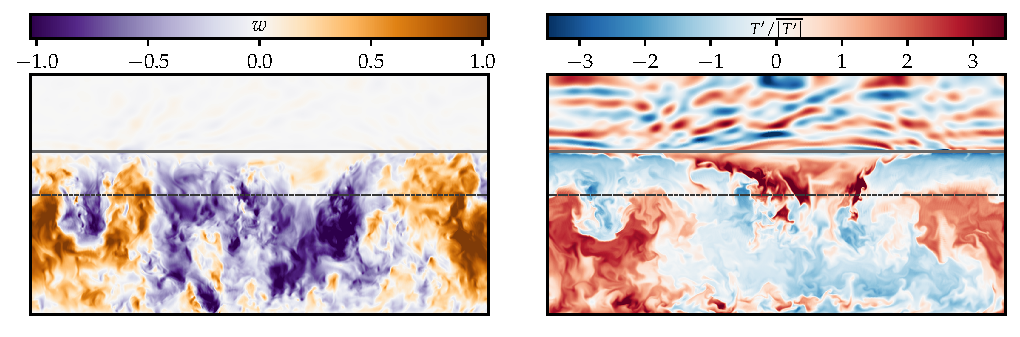
\includegraphics[width=\textwidth]{vertical_dynamics_panels.pdf}
\caption{
Instantaneous snapshots of a vertical slice through the simulation with $\mR = 3.2 \times 10^3$, $\mP_D = 4$ and $\mS = 10^3$ are shown.
In both panels, the nominal Schwarzschild top of the convection zone where $\gradad = \gradrad$ is displayed as a dashed horizontal line, and the top of the convection zone where $\grad$ departs from $\gradad$ by 10\% of $\Delta = \gradad - \gradrad$ is shown as a solid horizontal line.
(Left) The vertical velocity is shown; convective upflows extend far past the Schwarzschild boundary of the convection zone but stop abruptly where $\grad$ departs from $\gradad$.
(Right) Temperature perturbations away from $\overline{T}$ are shown; these perturbations are normalized by their standard deviation at each height in order to make both the convective features (below the solid black line) and internal gravity waves excited by the convection (above) visible.
Unlike in the vertical velocity slice, we see that the temperature perturbations switch sign at the Schwarzschild boundary of the convection zone (the dashed horizontal line); buoyancy thus switches from an accelerating force to a braking force.
\label{fig:vertical_dynamics_panels}
}
\end{figure}

In Fig.~\ref{fig:vertical_dynamics_panels}, we display instantaneous vertical slices through a turbulent simulation with $\mP_D = 4$ and $\mS = 10^3$ in an equilibrated state.
We see that strong convective dynamics (viewed in the left vertical velocity panel) extend beyond the Schwarzschild boundary of the convection zone into a penetration zone.
However, there is still a stable radiative zone with small vertical velocity perturbations into which the convection does not extend.
On the right, we see that hot upwellings in the convective dynamics are turned into cold upwellings in the PZ as a result of effective cooling from the sharp change in $k$ around the Schwarzschild boundary of the convection zone.
These upwellings impinge upon the stable radiative zone and excite gravity waves [cf., CITE], but our focus in this work is on the nature of the PZ where convective velocities and temperature anomalies are oppositely signed.

\subsection{Measured penetration zone scalings}

\begin{figure}[t!]
\centering
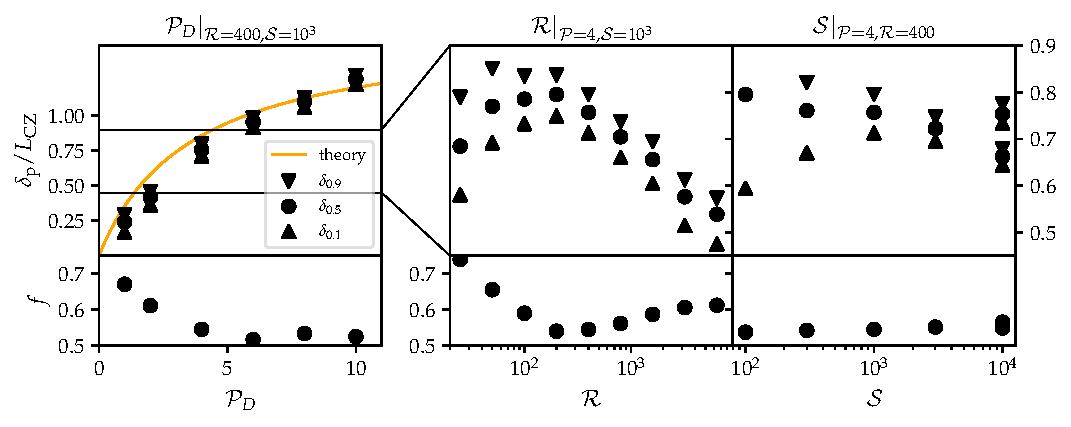
\includegraphics[width=\textwidth]{erf_3D_penetration_depths.pdf}
\caption{
We plot penetration depths against $\mP_D$ (left, at constant $\mR$, $\mS$), $\mR$ (center, at constant $\mP_D$, $\mS$), and $\mS$ (right, at constant $\mP_D$, $\mR$).
Up-triangles are the location of 10\% departure, down-triangles are the location of 90\% departure, and circles are the location of 50\% departure.
In the left panel, we plot a line corresponding to the theory of Eqn.~\ref{eqn:discontinuous_prediction}.
We find that the penetration depth is a strong, roughly linear function of $\mP_E$, in good agreement with the theory.
The horizontal lines in the left panel represent the full range of the right two panels; the effects of varying $\mS$ and $\mR$ are secondary to the effects of $\mP$.
In the center panel, we see that the penetration depth increases at low $\mR$ as laminar dynamics give way to time-evolving dynamics.
As we increase the turbulence, the penetration depth decreases weakly and appears to asymptote in the turbulent regime.
In the right panel, we see little change in the 50\% departure point, and we see that 10\% and 90\% departure points converge to the central point as a function of stiffness.
\label{fig:erf_3D_penetration_depths}
}
\end{figure}

In Fig.~\ref{fig:erf_3D_penetration_depths}, we plot measured values of the penetration depth from Case I (discontinuous $k$) simulations, quantified by the 10\%, 50\%, and 90\% departure points from $\gradad$.
In the left panel we plot the predicted scaling with $\mP_D$ from Eqn.~\ref{eqn:discontinuous_prediction} as well as the measured penetration depths from our simulations.
We find good agreement with the theory, and at large values of $\mP_D$ find equilibrated states in which the PZ is equal to or greater in size than the nominal convection zone (of unit depth).
We find that the value of $\mP_D$ is the primary parameter whose value modifies the height of the convection zone.
While not presented in this work, we performed limited 2D simulations and found similar scalings, but with larger penetration zones for the same parameters in 2D than in 3D.

In the center and rightmost panels of Fig.~\ref{fig:erf_3D_penetration_depths}, we focus on modifications to the measured penetration depths achieved by varying $\mR$ (turbulence) and $\mS$ (stiffness).
We find that the penetration depth is smaller at very low (laminar) values of $\mR$ and at high (turbulent) values of $\mR$, with a peak at moderate values (for which dynamics are interesting and non-stationary, but not as turbulent as e.g., Fig.~\ref{fig:vertical_dynamics_panels}).
Our data suggest that the penetration depth asymptotes as $\mR$ increases and so our results should be relevant for the astrophysical case in which $\mR \rightarrow \infty$.
We note however that these simulations are expensive to run and cannot be converged to the same degree of confidence as the simulations for which $\mR \lesssim 10^3$, which we run for thousands of overturn times.
We find that mean penetration depth (the 50\% departure point) shows little dependence on the stiffness (circles in the right panel).
However, the depth of the transition region from the PZ to the RZ shows a strong dependence on stiffness.
In stars, the stiffness is roughly determined by the Mach number ($\rm{Ma}^{-2} \sim \mS$), so for low-Mach convective stellar flows, the boundary of the PZ and RZ can likely be reasonably approximated as a step function in $\grad$.

\begin{figure}[t!]
\centering
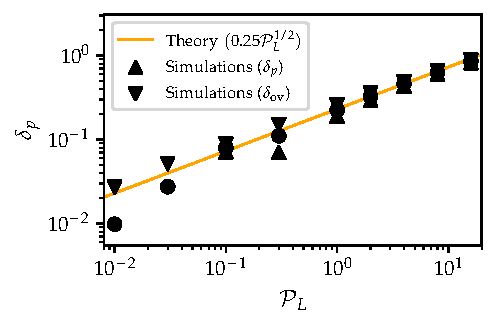
\includegraphics{linear_3D_penetration_depths.pdf}
\caption{
Similar to Fig.~\ref{fig:erf_3D_penetration_depths}, but for the Case II ``linear'' simulations where the slope of $k$ is discontinuous at the Schwarzschild point.
We plot a line corresponding to the theory of Eqn.~\ref{eqn:linear_prediction} as well as the 10\% (up triangle), 50\% (circle), and 90\% (down triangle) departure points.
We find that the theory describes our simulation measurements well.
We note that at small values of $\mP_L \lesssim 10^{-1}$, the 10\% departure point approaches the Schwarzschild boundary of the convection zone, approaching zero and not appearing on this plot.
\label{fig:linear_3D_penetration_depths}
}
\end{figure}

Finally, in Fig.~\ref{fig:linear_3D_penetration_depths}, we plot penetration depths as a function of $\mP_L$ for the ``linear'' Case II simulations.
We compare these depths to the theory of Eqn.~\ref{eqn:linear_prediction}.
We hold $\mR = 800$ and $\mS = 10^3$ constant for these simulations.
As in the discontinuous simulations, we find excellent agreement between the simulations and the theory.

Our simulation results present a strong case for the validity of \citet{zahn1991}'s theory.
The generalized Eqn.~\ref{eqn:theory_fraction}, and its solution for our simulation setups in Eqns.~\ref{eqn:discontinuous_prediction} \& \ref{eqn:linear_prediction}, describe our data well.
In addition to the flux-based penetration parameter $\mP$, the theory of Eqn.~\ref{eqn:theory_fraction} depends on the horizontal structure of the flux-carrying convective flows.
In this work, from the theory lines plotted in Figs.~\ref{fig:erf_3D_penetration_depths} \& \ref{fig:linear_3D_penetration_depths}, we find
\begin{equation}
\frac{(\overline{h}^3/\overline{h^2})_{\rm{PZ}}}{(\overline{h^3}/\overline{h^2})_{\rm{CZ}}} \approx 0.125 \,\,(\text{Case I: Discontinuous}),\qquad
\frac{(\overline{h}^3/\overline{h^2})_{\rm{PZ}}}{(\overline{h^3}/\overline{h^2})_{\rm{CZ}}} \approx 0.0625 \,\,(\text{Case II: Linear}).
\end{equation}
As the case II linear simulations are more applicable in the regime of stellar convection, we suggest that those simulations likely provide a starting guess for how to implement \citet{zahn1991}'s theory in 1D stellar models.
We examine this further in the next section.











\section{A modified solar model}
\label{sec:solar_model}

\section{Discussion}
\label{sec:discussion}

\begin{acknowledgments}
We'd like to thank
\end{acknowledgments}


\appendix

\section{Accelerated Evolution}
\label{app:accelerated_evolution}
\citet{anders_etal_2018}

\section{Table of simulation parameters}
\label{app:simulation_table}





\bibliographystyle{aasjournal}
\bibliography{biblio}
\end{document}
